\chapter*{Conclusões}\label{cap:conclusao}
Aqui serão abordados as conclusões da pesquisa referentes aos resultados do capítulo ~\ref{cap:resultados},  bem como uma sessão de Trabalhos Futuros e um Cronograma. Em Trabalhos Futuros a pretenção é expor melhoriras e expansões de tudo que fora realizado  nesta pesquisa, e mostrar que existe uma continuidade para todo esse estudo aqui elaborado. Já no Cronograma, será criado uma tabela divida em meses definindo os passos a serem seguidos até a conclusão da dissertação.

\section*{Conclusões}
\addcontentsline{toc}{section}{Conclusões}

O que se pretende fazer aqui nesta sessão é comentar as conclusões aqui realizadas neste trabalho, capítulo ~\ref{cap:resultados}, onde nesse capítulo mostrou a aplicação dos algoritmos supervisionados em cima de algumas bases de dados, e de fato reletar se o objetivo foi satisfatório, ou não.

Uma vez conhecido o problema, foi realizado a execução de dois algoritmos supervisionados, servindo de amostra para provar que era possível fazer rotulação de dados com quaisquer algoritmos supervisionados, tema deste trabalho. E já identificando alguns trabalhos que já haviam feito rotulação, ~\cite{Lopes}, utilizando algoritmos supervisionados, o intuito era executar outros algoritmos com paradigmas diferentes aos que foram realizados em pesquisas anteriores. 

Dos dois algoritmos apresentados, um pertencente ao paradigma simbólico e o outro estatístico. Além do que cada execução deles resultaram em respostas satisfatórias no âmbito da rotulação de dados. Embora cada um tenha suas peculiaridade.

No modelo de resolução proposto foi inicialmente utilizado Naive Bayes na base de dados Seeds\footnote{Sessão ~\ref{cap:resultados:ssec:seed:nb}}. Logo o resultado mostrou-se bem confiável pois o método consegue mostrar através da tabela ~\ref{tab:execucoes:seed:nb}, os valores de correlação entre os atributos, também exibido na coluna \textbf{Relevância} da tabela \ref{tab:rot:seeds:nb}. Dessa forma fica fácil identificar quais os atributos podem ser os rótulos dos clusters. Embora essa decisão possa ser modificada de acordo com o valor da variável ${V}$. Variável criada para melhor escolher os atributos do rótulo, a qual dependente do comportamento da base de dados.

Continuando com a base Seeds, após a escolha do atributo que fará parte do rótulo, o segundo passo é a escolha da faixa de valores do atributo. Essa segunda etapa é dependente totalmente da discretização\footnote{sessão ~\ref{cap:refTeor:sec:discret}} e independente da primeira etapa. O método é capaz de gerar a faixa de maior repetição de valores de qualquer atributo, mas aqui neste trabalho escolhemos o atributo rótulo. Para ter mais  confiabilidade  no rótulo o método escolhe a faixa de valores que mais se repetem. No caso desse algoritmo o resultado na tabela \ref{tab:rot:seeds:nb} consegue provar uma boa eficiência, pois em cada 70 elementos do cluster 1, somente 14, ficaram de fora dessa faixa. No cluster 2, somando os dois atributos rótulos tem-se 12 elementos que não estão dentro da representatividade do rótulo. Outro valor pequeno em relação aos 70 elementos. E no cluster 3, somente 5 elementos não estão dentro da faixa considerada rótulo.


\begin{figure}[h!]
    \centering
    \subfloat[Naive Bayes]{
        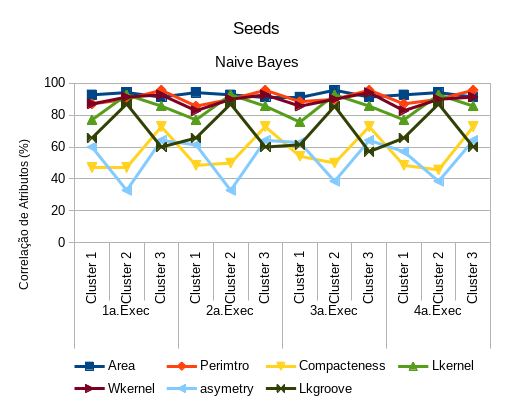
\includegraphics[scale=0.5]{figs/grafico_NB_SEED_exec_grp.png}
        \label{fig:execucoes:nb} }
    \quad
    \subfloat[CART]{
        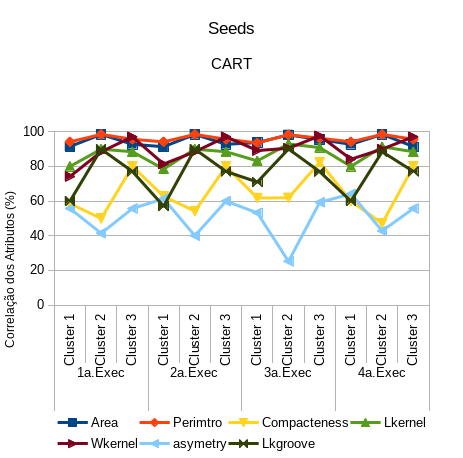
\includegraphics[scale=0.5]{figs/grafico_CART_SEED_exec_grp.png}
        \label{fig:execucoes:cart} }
    
    \caption{Gráfico de Execuções dos algoritmos supervisionados na base de dados Seed.} \label{fig:graf:SEED_NB_CART}
        
        %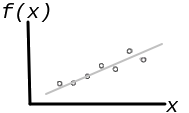
\includegraphics[scale=0.4]{figs/grafB.png}
        %\caption{Polinômio Superajustado} \label{grafB}
\end{figure}


No caso do algoritmo CART, os resultados foram diferentes dos  apresentados pelo Naive Bayes, mas nem por isso foram insatisfatórios. Contudo uma breve análise sobre as execuções das tabelas ~\ref{tab:execucoes:seed:nb} e \ref{tab:execucoes:seed:cart} podem ser observadas nos gráficos da figura ~\ref{fig:graf:SEED_NB_CART}. Como já comentado anteriormente o comportamento dos valores do correlecioanamento dos atributos ao longo das execuções mostra-se equilibrada, figura ~\ref{fig:execucoes:cart}. O gráfico tem um movimento semelhante ao do ~\ref{fig:execucoes:nb}, embora a variável \textbf{asymetry} saia um pouco do padrão, mas como seus valores são baixos, nada alterou nos rótulos , contudo  o valor de \textbf{perimetro} ficou bastante encostado ao valor da \textbf{area}, fazendo com que o rótulo \textbf{perimetro} aparecesse nos grupos 1 e 2. E só não foi selecionado também no grupo 3 , pois  a variável \textbf{Wkernel} estava sempre com valores mais altos em todos as execuções do grupo 3.

De acordo com o que foi exposto acima pode-se dizer em análise, que o Naive Bayes acabou tendo resultados um pouco melhores, pois no quesito de elementos que estão fora da faixa definida pelo rótulo, o CART, acabou por ter valores maiores que os resultados do Naive Bayes. Resultando em mais elementos fora da faixa definida pelo rótulo. Quer dizer que o rótulo deixa de representar mais elementos usando o CART ao invés do Naive Bayes, ou em outras palavras, o Naive Bayes representa mais elementos que o CART.



\section*{Trabalhos Futuros}
\addcontentsline{toc}{section}{Trabalhos Futuros}

\lipsum[85] 

\section*{Cronograma}
\addcontentsline{toc}{section}{Cronograma}

\lipsum[85] 
